\documentclass[10pt]{article}

%Math
\usepackage{amsmath}
\usepackage{amsfonts}
\usepackage{amssymb}
\usepackage{amsthm}
\usepackage{ulem}
\usepackage{stmaryrd} %f\UTF{00FC}r Blitz!

%PageStyle
\usepackage[ngerman]{babel} % deutsche Silbentrennung
\usepackage[utf8]{inputenc} 
\usepackage{fancyhdr, graphicx}
\usepackage[scaled=0.92]{helvet}
\usepackage{enumitem}
\usepackage{parskip}
\usepackage[a4paper,top=2cm]{geometry}
\setlength{\textwidth}{17cm}
\setlength{\oddsidemargin}{-0.5cm}


% Shortcommands
\newcommand{\Bold}[1]{\textbf{#1}} %Boldface
\newcommand{\Kursiv}[1]{\textit{#1}} %Italic
\newcommand{\T}[1]{\text{#1}} %Textmode
\newcommand{\Nicht}[1]{\T{\sout{$ #1 $}}} %Streicht Shit durch

%Arrows
\newcommand{\lra}{\leftrightarrow} 
\newcommand{\ra}{\rightarrow}
\newcommand{\la}{\leftarrow}
\newcommand{\lral}{\longleftrightarrow}
\newcommand{\ral}{\longrightarrow}
\newcommand{\lal}{\longleftarrow}
\newcommand{\Lra}{\Leftrightarrow}
\newcommand{\Ra}{\Rightarrow}
\newcommand{\La}{\Leftarrow}
\newcommand{\Lral}{\Longleftrightarrow}
\newcommand{\Ral}{\Longrightarrow}
\newcommand{\Lal}{\Longleftarrow}

% Code listenings
\usepackage{color}
\usepackage{xcolor}
\usepackage{listings}
\usepackage{caption}
\DeclareCaptionFont{white}{\color{white}}
\DeclareCaptionFormat{listing}{\colorbox{gray}{\parbox{\textwidth}{#1#2#3}}}
\captionsetup[lstlisting]{format=listing,labelfont=white,textfont=white}
\lstdefinestyle{JavaStyle}{
 language=Java,
 basicstyle=\footnotesize\ttfamily, % Standardschrift
 numbers=left,               % Ort der Zeilennummern
 numberstyle=\tiny,          % Stil der Zeilennummern
 stepnumber=5,              % Abstand zwischen den Zeilennummern
 numbersep=5pt,              % Abstand der Nummern zum Text
 tabsize=2,                  % Groesse von Tabs
 extendedchars=true,         %
 breaklines=true,            % Zeilen werden Umgebrochen
 frame=b,         
 %commentstyle=\itshape\color{LightLime}, Was isch das? O_o
 %keywordstyle=\bfseries\color{DarkPurple}, und das O_o
 basicstyle=\footnotesize\ttfamily,
 stringstyle=\color[RGB]{42,0,255}\ttfamily, % Farbe der String
 keywordstyle=\color[RGB]{127,0,85}\ttfamily, % Farbe der Keywords
 commentstyle=\color[RGB]{63,127,95}\ttfamily, % Farbe des Kommentars
 showspaces=false,           % Leerzeichen anzeigen ?
 showtabs=false,             % Tabs anzeigen ?
 xleftmargin=17pt,
 framexleftmargin=17pt,
 framexrightmargin=5pt,
 framexbottommargin=4pt,
 showstringspaces=false      % Leerzeichen in Strings anzeigen ?        
}

%Config
\renewcommand{\headrulewidth}{0pt}
\setlength{\headheight}{15.2pt}

%Metadata
\fancyfoot[C]{If you use this documentation for a exam, you should offer a beer to the authors!}
\title{
	\vspace{5cm}
	Aplikationssicherheit
}
\author{Jan Fässler \& Ege Kaba}
\date{5. Semester (HS 2013)}


% hier beginnt das Dokument
\begin{document}

% Titelbild
\maketitle
\thispagestyle{fancy}

\newpage

% Inhaltsverzeichnis
\pagenumbering{Roman}
\tableofcontents	  	


\newpage
\setcounter{page}{1}
\pagenumbering{arabic}

% Inhalt Start

\section{SSL}
\subsection{The secure channel}
\begin{itemize}
	\item A, B key-exchange protocol that establishes an \textbf{Authenticated, Secret Session Key} between A and B
	\item This \textbf{session key }is used together with a \textbf{symetric key} cryptographic function to protect the \textbf{integrity} and/or \textbf{secrecy} of the transmitted data.
\end{itemize}
\subsection{security in the TCP/IP stack}
\begin{center}
	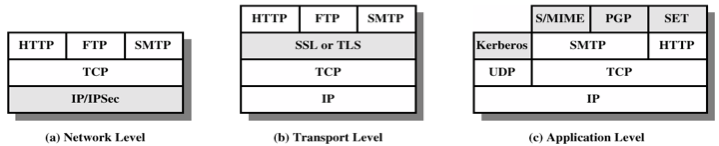
\includegraphics[scale=0.5]{ssl_in_tcpip.png}
\end{center}
\subsection{diffrent parts of the SSL protocoll}
\begin{center}
	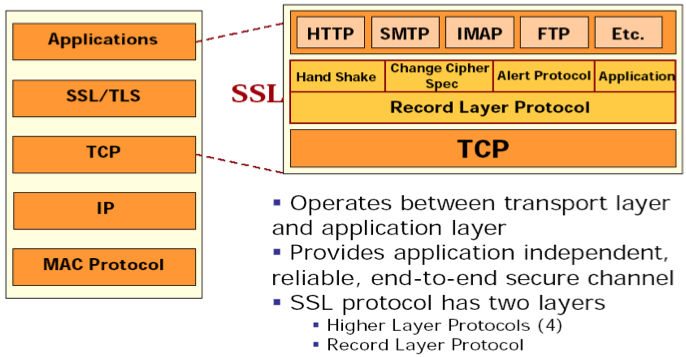
\includegraphics[scale=0.5]{ssl_diffrent_parts.png}
\end{center}
\subsection{SSL(TLS) over TCP/IP}
\begin{center}
	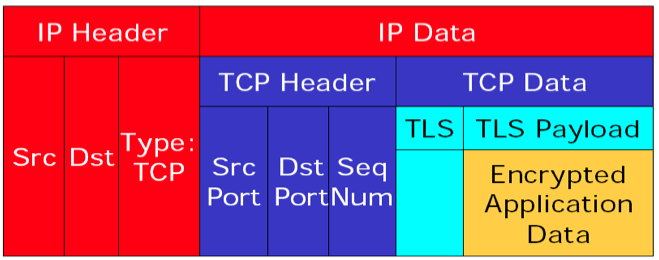
\includegraphics[scale=0.5]{ssl_tls.png}
\end{center}
\subsection{SSL characteristics}
\begin{itemize}
	\item Netscape Secure Socket Layer
	\item Layered between the application and TCP
	\item Server authenticated with public keys (X509)
	\item Can authenticate client (rare)
	\item Privacy enforced by encryption
	\item Integrity enforced by MACs
	\item Works with any TCP application
\end{itemize}
\subsection{SSL protocols}
SSL provides end to end security, based on a communication protocol. The different protocols implemented by SSL:
\begin{itemize}
	\item Handshake
	\item Record (specifies how the data are encrypted)
	\item Change cipher specifications
	\item Alert services
\end{itemize}
\subsection{Handshake protocol}
The ost complex and unsecure part of SSL are:
\begin{itemize}
	\item Allows the server and client (\textbf{optional}) to athenticate each other
	\item Negotiate encryption, message authentication code algorithm and cryptographic keys
	\item Used before any application data are transmitted
\end{itemize}
\subsubsection{SSL protocol basic handshake features}
\begin{enumerate}
	\item The client initiates the connection to the server and tells the server which SSL cipher suites the client supports.
	\item The server responds with the cipher suites that it supports.
	\item The server sends the client a certificate that should authenticate it.
	\item The server initiate a session key exchange algorithm, based in part on the information contained in the certificate it has just sent, and sends the necessary key exchange information to the client.
	\item The client completes the key exchange algorithm and sends the necessary key exchange information to the server. Along the way, it verifies the certificate.
	\item Based on the type of key exchange algorithm (that in turn is based on the type of key in the server’s certificate), the client selects an appropriate cipher suite and tells the server which suite it wishes to use.
	\item The server makes a final decision as to which cipher suite to use.
\end{enumerate}
\subsubsection{protocol gritty details}
\begin{center}
	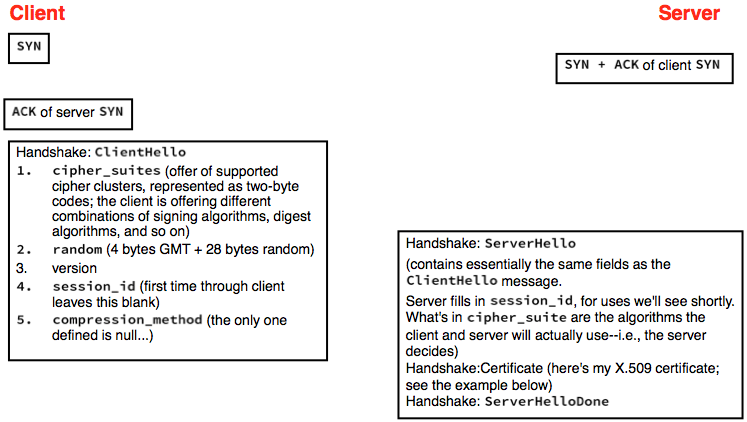
\includegraphics[scale=0.5]{handshake1.png}
	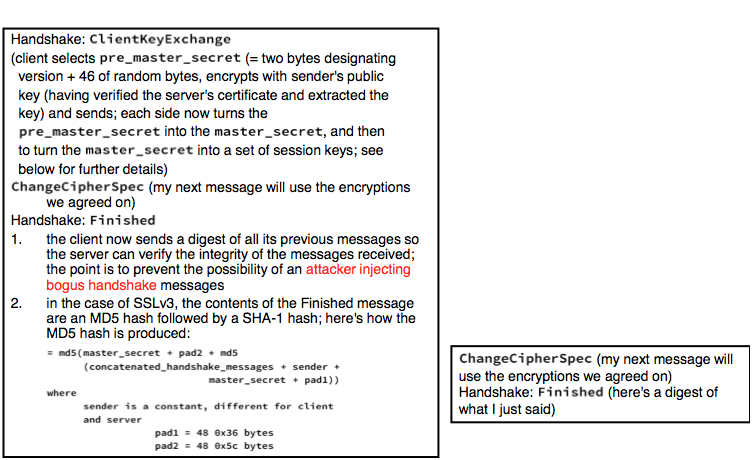
\includegraphics[scale=0.5]{handshake2.png}
	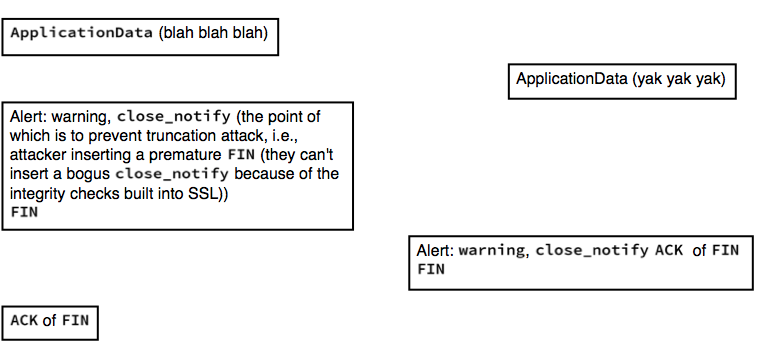
\includegraphics[scale=0.5]{handshake3.png}
\end{center}
\subsubsection{generating Master Secret}
\begin{center}
	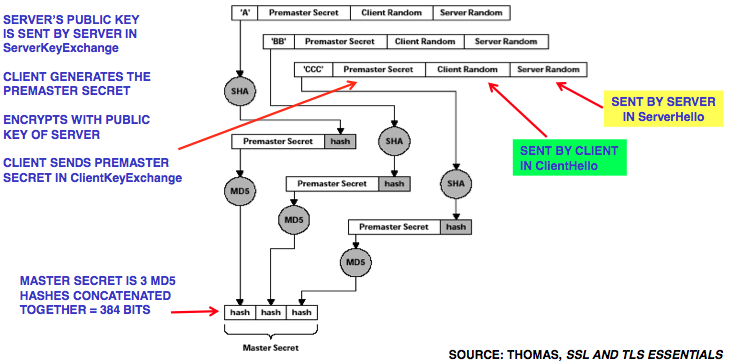
\includegraphics[scale=0.5]{ssl_master.png}
\end{center}
\subsubsection{generating key material}
\begin{center}
	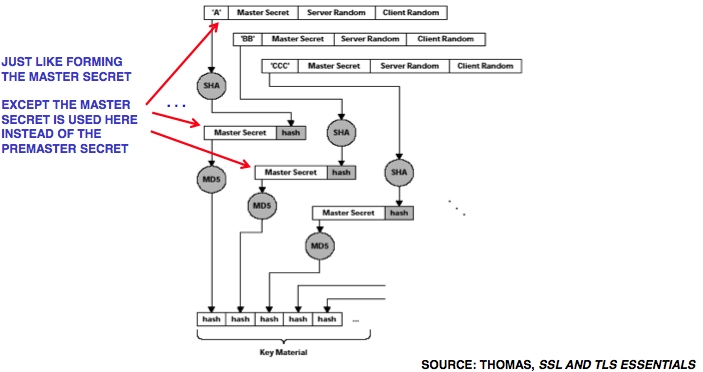
\includegraphics[scale=0.5]{ssl_key_materials.png}
\end{center}
\subsection{Record protocol}
\subsubsection{Ablauf}
\begin{enumerate}
	\item Provides confidentiality and integrity.
	\item Fragments message ( 214 bytes).
	\item Optional compression (default: none).
	\item Calculates MAC (Message Authentication Code = integrity). MAC traditionally is based on symmetric block cipher, i.e. MAC = CK(M) where M is the message, MAC a fixed length authenticator, K a secret symmetric key shared between sender and receiver and C(.) a function.
	\item Modified H(Hash)MAC to include sequence number (prevent replay attacks).
	\item Encrypts both message and MAC (confidentiality+integrity).
	\item Propend header.
\end{enumerate}
\subsubsection{Format}
\begin{center}
	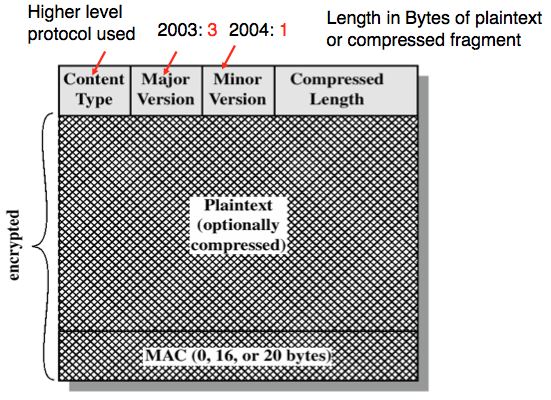
\includegraphics[scale=0.4]{ssl_record_format.png}
\end{center}
\subsection{SSL remaining protocols}
\begin{center}
	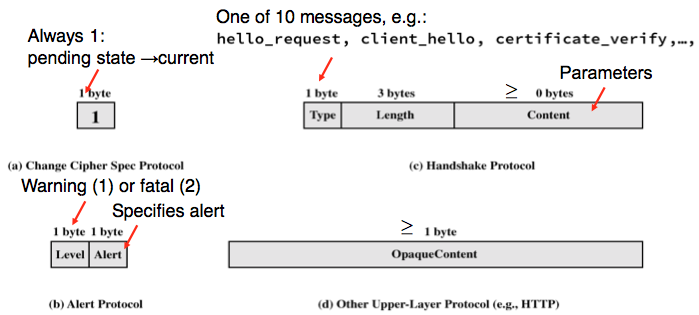
\includegraphics[scale=0.4]{ssl_remaining_protocols.png}
\end{center}
\subsection{TLS enhancements}
Differences in the:
\begin{itemize}
	\item version number
	\item message authentication code
	\item pseudorandomfunction(PRF)
	\item alert codes
	\item cipher suites
	\item client certificate types
	\item certificate\_verify and finished message
	\item cryptographic computations
	\item padding
\end{itemize}
Otherwise similar to SSL v3.1. Important: the same record format as the SSL record.
\subsection{Words to the wise about applied cryptography}
\begin{enumerate}
	\item Hashing and symmetric key ciphers are fast: use them for session encryption.
	\item RSA public key is slow, but it is useful for key exchange and user/server authentication
	\item Informal web of trust of PGP (you are in charge) versus CA based (you do not know, who controls it: in fact the NSA controls it (note added in 2013))
	\item A good protocol should:
		\begin{enumerate}
			\item negotiate \textbf{cryptographic} parameters
			\item establish \textbf{shared} secret
			\item authenticate \textbf{endpoints}
		\end{enumerate}
	\item Use ssh, pgp liberally as the crypto part of an application.
	\item SSL: a transport interface, but you still needs to modify the application
	\item IPsec places cryptography where it belongs: at the network layer.
\end{enumerate}
\subsection{SSL and Java applications}
\subsubsection{Java SSL software (JSSE)}
Set of API to construct SSL-Client and SSL-Server sockets. \\
Two important new concepts: \textbf{trust store} and \textbf{key store}. Both are databases that hold certificates. Key store are used to provide credentials; trust store to verify them.
\begin{center}
	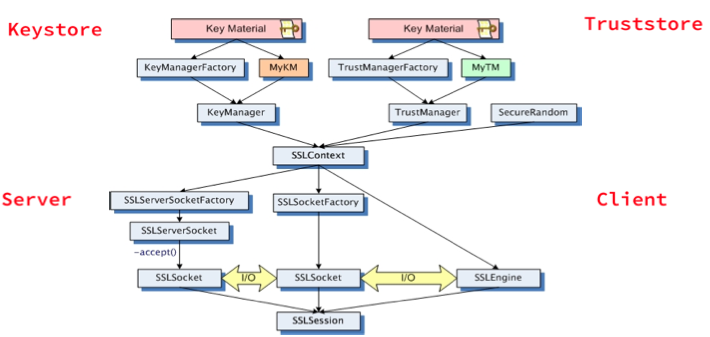
\includegraphics[scale=0.4]{ssl_class_diagram.png}
\end{center}
\subsubsection{X.509 certificate}
Every X.509 certificate consists of two sections: (i) data and (ii) signature. \\
The data section includes the following information:
\begin{enumerate}
	\item The v\textbf{ersion number} of the X.509 standard supported by the certificate.
	\item The certificate's \textbf{serial number}. Every certificate issued by a CA has a serial number that is unique to the certificates issued by that CA.
	\item Information about the user's \textbf{public key}, including the algorithm used and a representation of the key itself.
	\item The \textbf{DN} of the CA that issued the certificate.
	\item The period during which the certificate is \textbf{valid} (for example, between 1:00 p.m. on January 1, 2000 and 1:00 p.m. December 31, 2000).
	\item The DN of the certificate \textbf{subject} (for example, in a client SSL certificate this would be the user's DN), also called the subject name.
	\item Optional c\textbf{ertificate extensions}, which may provide additional data used by the client or server. For example, the certificate type extension indicates the type of certificate - that is, whether it is a client SSL certificate, a server SSL certificate, a certificate for signing email, and so on. Certificate extensions can also be used for a variety of other purposes.
\end{enumerate}
The signature section includes:
\begin{enumerate}
	\item The \textbf{cryptographic algorithm}, or cipher, used by the issuing \textbf{certificate authority (CA)} to create its own digital signature.
	\item The CA's \textbf{digital signature}, obtained by hashing all of the data in the certificate together and encrypting it with the CA's private key.
\end{enumerate}
\subsubsection{Webserver verification of client's certificate}
\begin{center}
	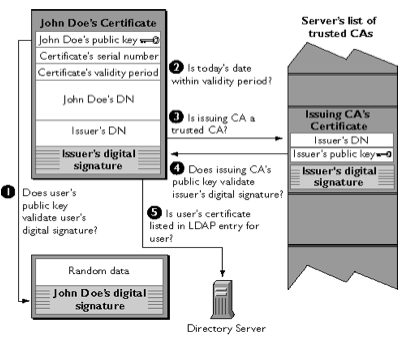
\includegraphics[scale=0.5]{ssl_server_verification.png}
\end{center}
\subsubsection{Client verification of server's certificate}
\begin{center}
	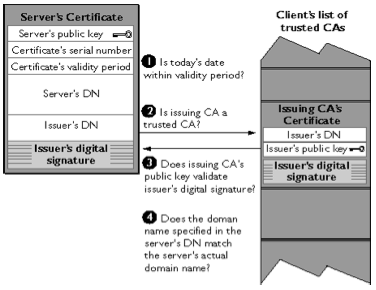
\includegraphics[scale=0.5]{ssl_client_verification.png}
\end{center}
\subsubsection{Certification path}
The chain, or path, begins with the certificate of that entity, and each certificate in the chain is signed by the entity identified by the next certificate in the chain. The chain terminates with a root CA certificate. The root CA certificate is always signed by the CA itself.
\subsubsection{A secure Webserver in Java}
\lstinputlisting[caption=secure webserver,style=JavaStyle]{ssl_server.java}

\newpage
\section{Validation}
\subsection{Fundamental principles}
\begin{enumerate}
	\item \textbf{Least privilege}: Both users and applications should have only the minimum set of privileges necessary to run.
	\item \textbf{Economy of mechanisms/Simplicity}: “Techniques such as line by line inspection of software and physical examination of hardware that implements protection mechanisms are necessary. For such techniques to be successful, a small and simple design is essential.”
	\item \textbf{Open design}: The protection mechanism must not depend on the attacker’s ignorance. Security by obfuscation is not only stupid, but dangerous too.
	\item \textbf{Complete mediation}: Every access attempt must be checked.
	\item \textbf{Fail-safe defaults}: The default should always be denial of access. The protection scheme should clearly identify under which conditions access is permitted.
	\item \textbf{Separation of privilege}: Access to objects should depend on more than one condition, so that defeating one protection’s layer doesn’t grant complete access. (Compartmentalisation.)
	\item \textbf{Least common set of mechanism}: Minimize the amount and use of shared mechanisms.
	\item \textbf{Easy to use}: If the protection is not intuitively simple to learn, the users will ignore it.
\end{enumerate}
\subsection{Points of attack}
\begin{center}
	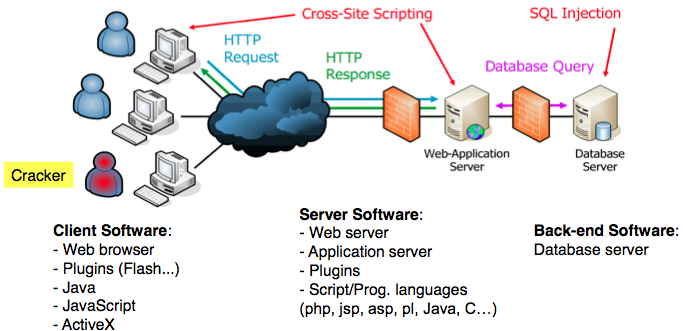
\includegraphics[scale=0.5]{points_of_attac.png}
\end{center}
\subsection{SQL injection}
\subsubsection{login attack}
The cracker (always aptly named Oscar) logs in:
\begin{itemize}
	\item He tries to manipulate the SQL query in such a way that it always returns at least one row.
	\item With logins, this often works with 'or' '='
	\item GET/path/login.pl?user='or''='\&pwd='or''='HTTP/1.0
	\item Resulting SQL query: SELECT * FROM Users WHERE users='' or ''='' AND pwd='' or ''=''
	\item Since the WHERE clause is always true, the query returns all rows
	\item The attacker is allowed to “enter the system” and gets the identity of the first entry in the table Users
\end{itemize}
\subsubsection{some more tricks}
Suppose users can select car models via a drop-list:
\begin{itemize}
	\item Selected entry is sent as a number to the web server
	\item GET/path/showcars.pl?brand\_id=17; DROP TABLE Users HTTP/1.0
	\item Resulting SQL query: SELECT * FROM Cars WHERE brandID=17; DROP TABLE Users
\end{itemize}
SQL injection is powerful, but it is not always easy to carry out:
\begin{itemize}
	\item One must first find out a vulnerable web application
	\item The internal structure of the database is normally unknown to the attacker
	\item The type of database the application uses, is mostly unknown
	\item Requires a good knowledge of SQL and of different database products
	\item Resulting SQL queries must be syntactically correct
\end{itemize}
\textbf{Good strategy}: \\
Insert a '(single quote) in web form fields: This usually breaks the SQL statements and (if we are lucky) gives information about the SQL via an error message;
\subsubsection{Defenses against SQL injection}
\begin{itemize}
	\item On the server, \textbf{validate}, \textbf{constrain} and \textbf{sanitize} all data provided by the client (length restriction, disallow critical characters (single quote etc.))
	\item Do not use client parameters directly in SQL queries, but use prepared statements (type-checking, parameters are escaped by the DBMS, only one query is executed)
	\item A similar effect can be achieved by parameterized stored procedures
	\item Avoid disclosing detailed database error information to the client
	\item Access the database with \textbf{minimal} privileges
\end{itemize}
\subsubsection{SQL statements’ sanitation}
\begin{lstlisting}[caption=PreparedStatement Pseudocode,style=JavaStyle]
updateSales = con.prepareStatement("UDATE Cars SET Name = ? WHERE id = ?");
updateSales.setString(1, e.getKey());
updateSales.setInt(2, e.getValue().intValue());
\end{lstlisting}
\subsection{Cross-Site Scripting}
\subsubsection{XSS}
Dynamically generated web pages send often data entered by the user in web forms back to the user. With XSS, an attacker exploits formulars:
\begin{itemize}
	\item The attacker submits a JavaScript in a web form
	\item The dynamically generated web page contains the script
	\item When displayed in a browser, the script is executed
	\item Unlike SQL injection, the attack targets another user, not the server!
	\item Effective attack because (i) most browsers have JavaScript enabled and (ii) it is platform independent
\end{itemize}
If an attacker manages to execute JavaScript code in the browser of a victim, the following is possible:
\begin{itemize}
	\item He can fetch arbitrary additional JavaScript code from a server
	\item He can retrieve the currently used session-id, which allows to take over the session by session hijacking (e-Commerce, e-Banking...)
	\item He can dynamically adapt the web page during the loading/rendering process in the victim’s browser, e.g. to replace the login dialogue with an own version and to steal the victim’s credentials
\end{itemize}
Difficulties for the attacker: To execute a JavaScript in the browser of another user, that user must send the JavaScript to the vulnerable web server
\subsubsection{Defenses against XSS}
Secure communication protocols, packet-filtering firewalls are useless. But: using HTTPS helps against Session Hijacking. \\
\textbf{Server side}: do the following:
\begin{itemize}
	\item Validate all data provided by client
	\item Sanitize all client-provided data before sending them back to the browser
	\item Especially watch for $<$script$>$, $<$/script$>$, javascript:
	\item Replace $<$ and $>$ around script of client-provided data with and browser interprets this as string literals and not as scripts
\end{itemize}
\textbf{Client side}: disable JavaScript
\subsection{Regular Expressions}
\subsubsection{Cheet Sheet}
\begin{center}
	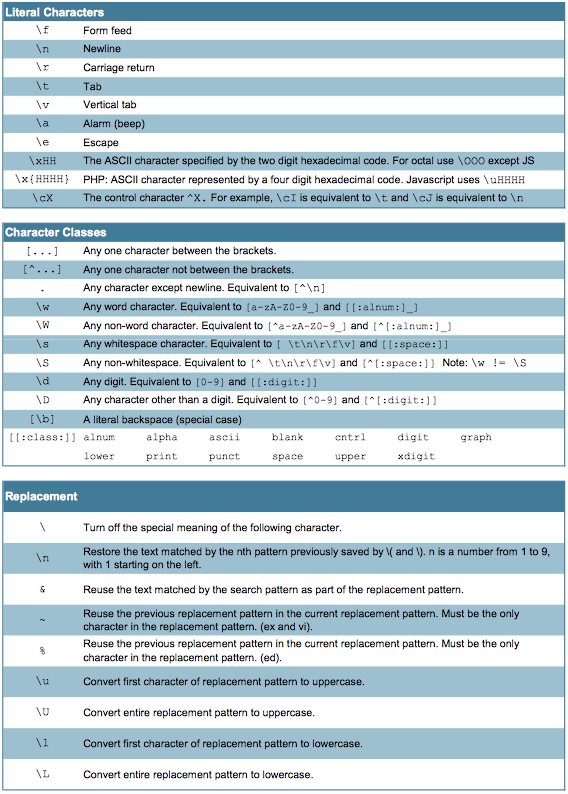
\includegraphics[scale=0.75]{regex1.png}
\end{center}
\begin{center}
	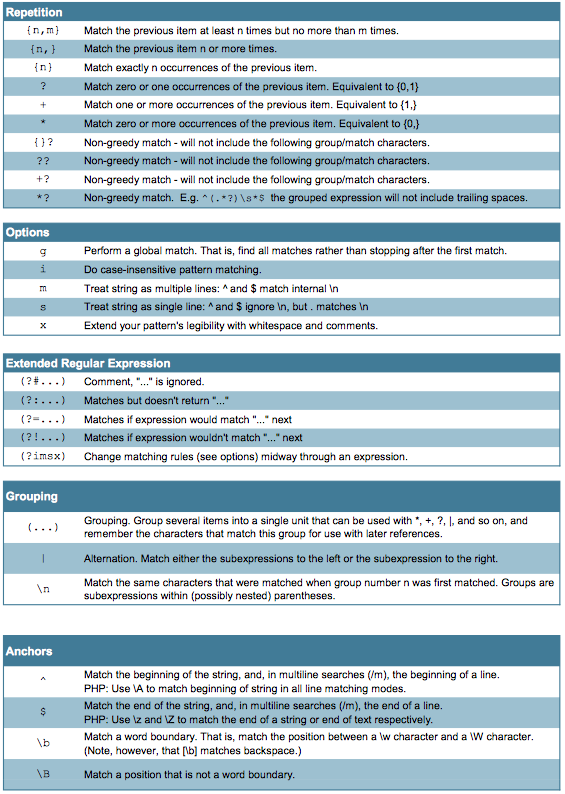
\includegraphics[scale=0.75]{regex2.png}
\end{center}
\subsubsection{Example}
\lstinputlisting[caption=email checker,style=JavaStyle]{regex.java}

\newpage
\section{Robust Programming}
\subsection{Einleitung}
Writing programs is not a trivial task. Most (large) programs that are written contain errors: that means that the program doesn't do what it's meant to do. \\
\\
There are many sources of error:
\begin{itemize}
	\item \textbf{Syntactic errors} (good compilers take care of that);
	\item \textbf{Semantic errors} (our brains are not perfect programming machines ...)
	\item Programs are "correct" but \textbf{input/output fail} and resource are not ready ! exception handling.
	\item \textbf{Languages' ambiguous specifications }(or their implementations) break the program (example: Java memory model and concurrency).
\end{itemize}
A good definition of robustness is therefore: \textbf{Graceful behaviour in presence of errors} \\
This means that if the program fails, it falls into a well known state and at least logs why it has failed.
\subsection{Specific tools enhance robustness}
The most useful techniques are:
\begin{itemize}
	\item Judicious use of types and visibility attributes;
	\item Annotations (compile time);
	\item Correct use of the exception handling mechnisms (run time);
	\item Assertions (run time).
\end{itemize}
\subsection{Types and visibility in Java}
\begin{description}
	\item[Rule 1] All fields are \textbf{private}
	\item[Rule 2] Fields, once initialized by the class constructor, are \textbf{never} updated.
\end{description}
Rule 1 + Rule 2 $\rightarrow$ the class is \textbf{immutable}!
\subsection{Code inheritance breaks encapsulation}
Against code inheritance:
\begin{enumerate}
	\item Strong relationship between base and derived class
	\item The extension of a class with sub classing, requires an in-depth knowledge about the implementation of the base class
	\item Specialization interface means:
		\begin{itemize}
			\item Protected methods: Disrupts the private/public only model.
			\item Specialization semantics
		\end{itemize}
\end{enumerate}
Inheritance breaks encapsulation: Support for inheritance implies that (some) implementation details have to be published!
\subsubsection{Instead inheritance use composition}
The advantages of composition:
\begin{itemize}
	\item Only the client interface is used
	\item No call-backs (in contrast to the inheritance based solutions)
	\item No dependency on the implementation
\end{itemize}
\subsubsection{Instead inheritance use Template/Hooks}
Template methods:
\begin{itemize}
	\item Template method pattern provides a robust method to allow for extensions
	\item Base class provides extension points
\end{itemize}
\subsection{Annotations}
\subsubsection{General remarks}
Annotations provide data about a program that is not part of the program itself. They have no direct effect on the operation of the code they annotate. \\
Main usages:
\begin{itemize}
	\item \textbf{Information for the compiler}: Annotations can be used by the compiler to detect errors or suppress warnings.
	\item \textbf{Compiler-time and deployment-time processing}: Software tools can process annotation information to generate code, XML files, and so forth.
	\item \textbf{Runtime processing}: Some annotations are available to be examined at runtime.
\end{itemize}
\subsubsection{Why are annotations so important?}
\begin{enumerate}
	\item Annotations act mostly at compile-time: and this is a very good thing. We want to catch all of our subtle and not so subtle errors at compile time and not at run- time in front of an important customer ...
	\item Annotations can be extracted by external tools. Instead of looking for methods with a particular name or signature, retrieve all methods with a specific annotation.
	\item Annotations are like classes. They have a specific type. They can contain fields to store details.
	\item Meta-specifications for annotations include:
		\begin{enumerate}
			\item Where they can appear on (e.g. only on classes, or only on methods)
			\item A retention policy: when and where they are made available:
		\end{enumerate}
\end{enumerate}
\subsubsection{Overview}
\begin{center}
	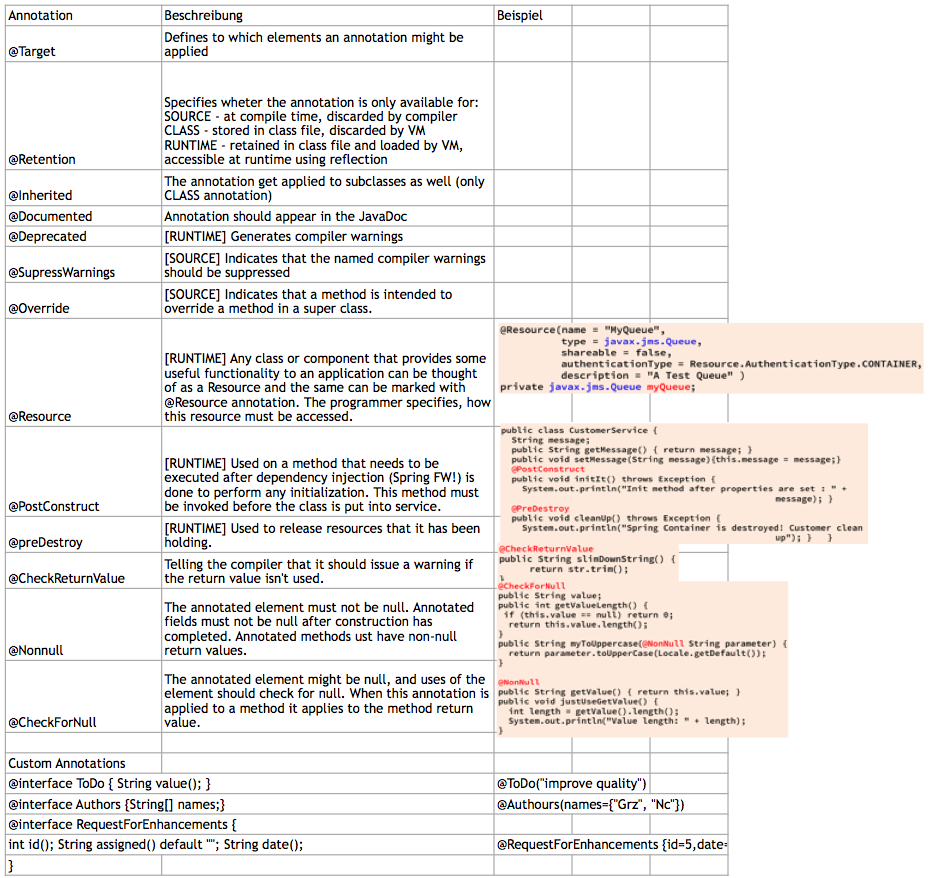
\includegraphics[scale=0.55]{annotations.png}
\end{center}
\subsection{exception handling}
\subsubsection{Ideal fault-tolerant software components}
\begin{center}
	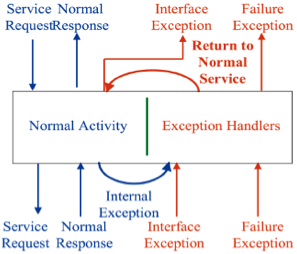
\includegraphics[scale=0.6]{fault_tolerant.png}
\end{center}
\subsubsection{Requirements for exception handling}
\begin{enumerate}
	\item \textbf{Simplicity}: Should be simple to understand and use
	\item \textbf{Unobtrusiveness}: Exception handling code should not obscure the understanding of the software: (1) and (2) are crucial for designing reliable systems!
	\item \textbf{Efficiency}: Run-time overheads should be incurred only when handling an exception. This may be relaxed, e.g. if speed of recovery is not critical
	\item \textbf{Uniformity}: Uniform treatment of exceptions detected both by the environment and by the program
	\item \textbf{Recovery}: It should allow recovery actions
\end{enumerate}
\subsubsection{Classes of exceptions}
Who detects the error?
\begin{itemize}
	\item Environmental error detection
	\item Application error detection
\end{itemize}
When it is detected?
\begin{itemize}
	\item \textbf{Synchronously}: as an immediate result of a process attempting an inappropriate operation
	\item \textbf{Asynchronously}: some time after the operation causing the error. May be raised either in the process which executed the operation or in another process. The latter is also called asynchronous notification or signal. Mostly an issue with concurrent programming.
\end{itemize}
\subsection{Assertions}
These three roles collectively support what is called the design-by-contract model of programming, a model that is well supported for example by the Eiffel programming language. Java doesn't have built-in support for the design-by-contract model of programming. But you can use the java.assertion package to enforce these rules.
\subsubsection{Decleration}
An assertion statement in Java takes one of the following two forms:
\begin{itemize}
	\item assert condition:
	\item assert condition : error message;
\end{itemize}
\subsubsection{enable/disable}
To enable assertions at various granularities, use the -enableassertions
To disable assertions at various granularities, use the -disableassertions

\newpage
\section{Action Control}
\subsection{Goal}
Specify the limits within which a legitimate user can work with the system.
\begin{center}
	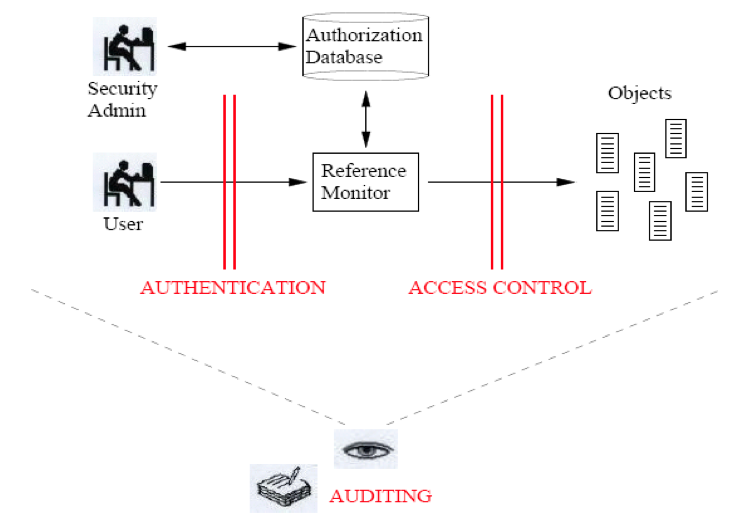
\includegraphics[scale=0.4]{action_control.png}
\end{center}
\subsection{AC policies}
Subjects detain privileges on objects according to AC policies (models). \\
\textbf{Policy}: specifies how accesses are controlled and access decisions determined. \\
\\
\textbf{Mechanism} (structure): implements or enforces a policy.
\begin{itemize}
	\item Access matrix.
	\item AC list (ACL).
	\item Capability list.
\end{itemize}
\subsubsection{Discretionary AC}
This policy restricts access to system objects based on the identity of the users and/or the groups to which they belong. \\
Two types of DAC policies are used in practice:
\begin{itemize}
	\item \textbf{Closed DAC}: authorization must be explicitly specified, since the default decision is always denial. 
	\item \textbf{Open DAC}: denials must be explicitly specified since the default decision is always access.
\end{itemize}
Problems:
\begin{itemize}
	\item Danger of users' mistakes or negligence;
	\item The dissemination of information is not controlled: for example a user who is able to read data can pass it to other users not authorized to read it without the actual owner knowing it.
\end{itemize}
\subsubsection{Mandatory AC}
Idea: each subject and each object is assigned a security level.
\begin{enumerate}
	\item Subject's label (clearance) specifies the level of trust associated with that subject.
	\item Object's label specifies the level of trust that a subject must have to be able to access that file.
\end{enumerate}
Pro: Reduction of possible damage \\
Contra: Loss of flexibility.
\subsection{Bell-LaPadula (BLP) policy model }
\begin{itemize}
	\item The Simple Security Policy: no process may read data at a higher level. \textbf{No Read Up (NRU)} or: a subject can only read an object of less or equal security level.
	\item The *-property: no process may write data to a lower level. \textbf{No Write Down (NWD) }or: a subject can only write into an object of greater or equal security level.
\end{itemize}
\begin{center}
	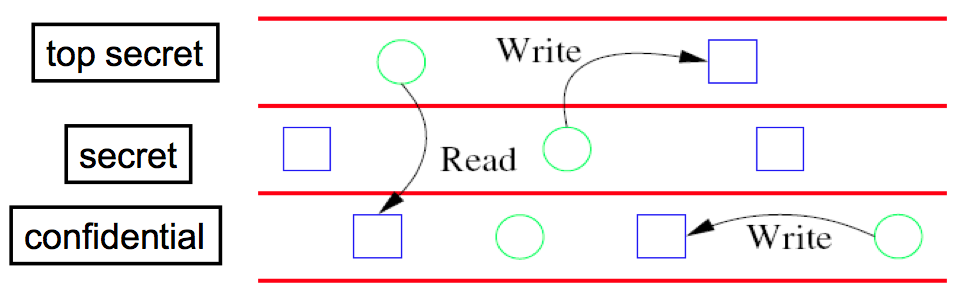
\includegraphics[scale=0.4]{bell-la_padula.png}
	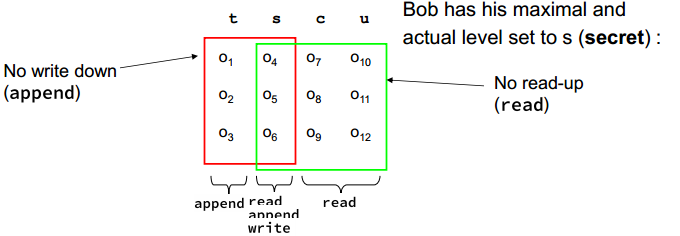
\includegraphics[scale=0.4]{bell-la_padula_eg.png}
\end{center}
\subsection{Other policy concepts}
\begin{itemize}
	\item Seperation of Duty: Check is only valid if signed y two authorized people
	\item Chinese Wall Policy
\end{itemize}
\subsection{Role-based access control (RBAC)}
Permissions are associated with:
\begin{itemize}
	\item roles  (= set of actions and responsibilities, associated with particular 
working activities)
	\item users/subjects
\end{itemize}
\subsection{ACM/ACL}
\begin{center}
	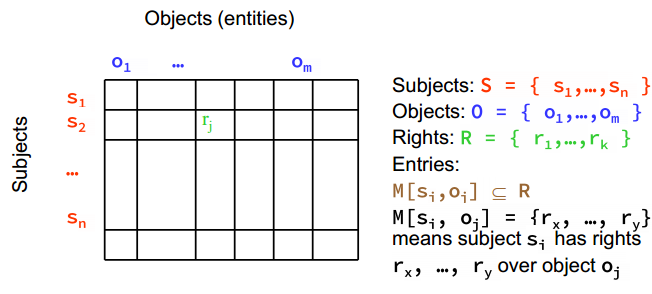
\includegraphics[scale=0.4]{acm.png}
\end{center}
Right to copy: Two rights in stead of one Read (r / rc).
Attenuation of privilege: You can't give away rights you do not possess. This principle is usually ignored for the owner of an object.
\textbf{Summary}
\begin{itemize}
	\item Access control matrix is the simplest abstraction  mechanism for representing a   protection state within a system.
	\item Transitions alter the protection state.
	\item Six primitive operations alter the AC matrix: Transitions can be expressed as commands composed of these operations and, possibly , conditions. 
\end{itemize}
\subsection{AC list (ACL)}
In large systems the matrix will be big and sparse.  Therefore in practice, the matrix is implemented as a list.
\begin{center}
	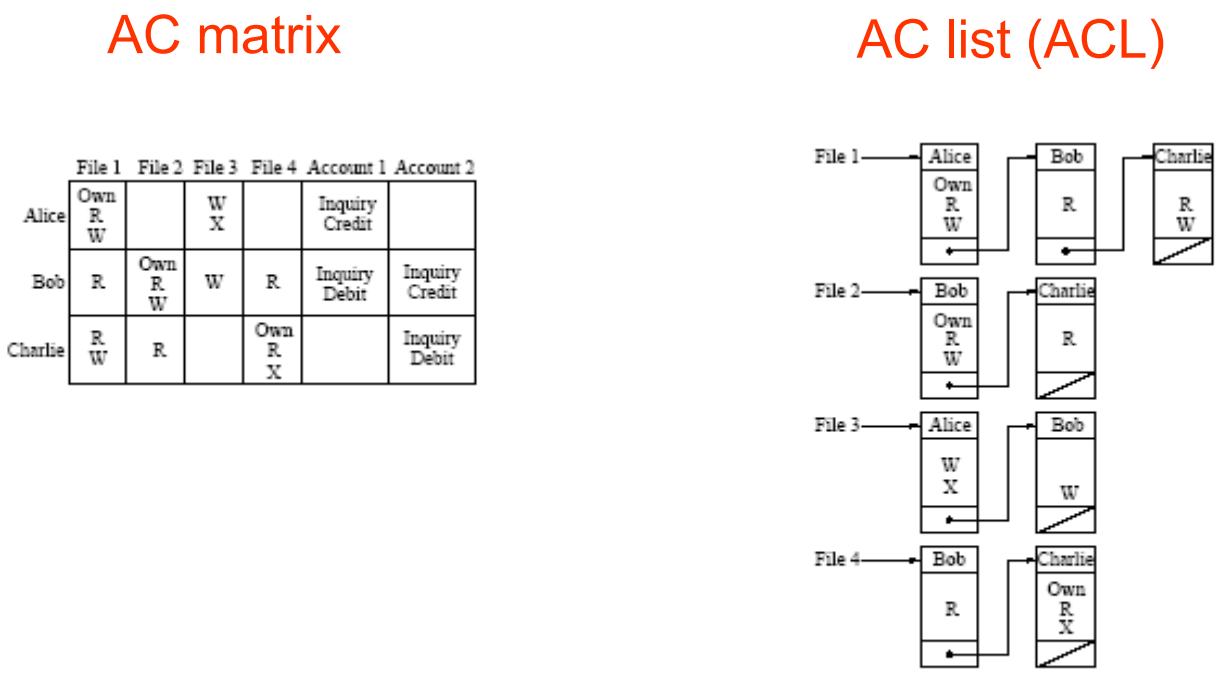
\includegraphics[scale=0.4]{acm_to_acl.png}
\end{center}
\subsection{Capability list}
\begin{center}
	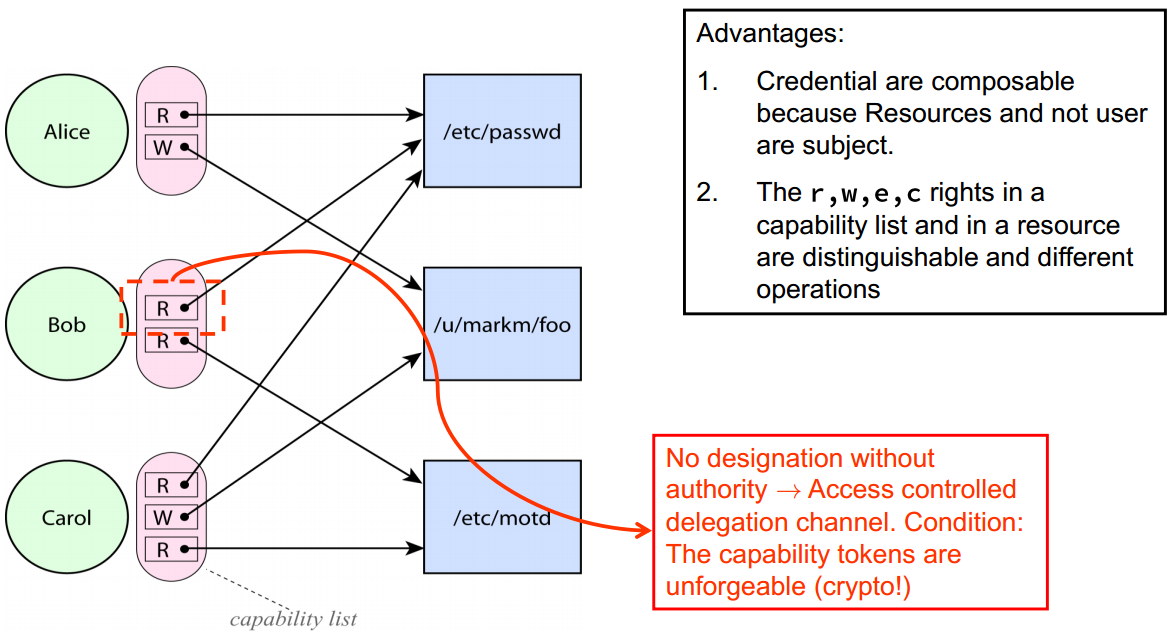
\includegraphics[scale=0.4]{capability_list.png}
\end{center}
\textbf{Delegation:} Process can pass capability at run time
\textbf{Revocation:}
\begin{itemize}
	\item Only if OS knows which data is associated with a capability. If capability is used for multiple resources, one has to revoke all or none.
	\item Indirection: capability points to pointer to resource (C=>P=>R, set P=0 to revoke)
\end{itemize}
\subsection{Android}
\subsubsection{Basic Components of an Application}
\begin{itemize}
	\item Activity: User Interface
	\item Service: Java daemon
	\item Content provider: Store and share data
	\item Broadcast receiver: For messages from other applications
	\item Intents: asynchronous mesaging system
\end{itemize}
\subsubsection{Security steps}
\begin{itemize}
	\item Signing with certificates
	\item Application sandbox: runs with its UID and own Dalvik virtual machine
	\item Linux and ACL
	\begin{itemize}
		\item Each application executes with its own user identity as Linux process
		\item Android middleware has a reference monitor that mediates the establishment of inter-component communication (ICC)
	\end{itemize}
\end{itemize}
\subsubsection{Android manifest file}
Focus on Inter Component Communication (ICC) whose security policy is defined in the Android manifest file. Allows developers to specify a high-level ACL to access the components:
\begin{itemize}
	\item Each component can be assigned an access permission label
	\item Each application requests a list of permission labels
\end{itemize}
\begin{center}
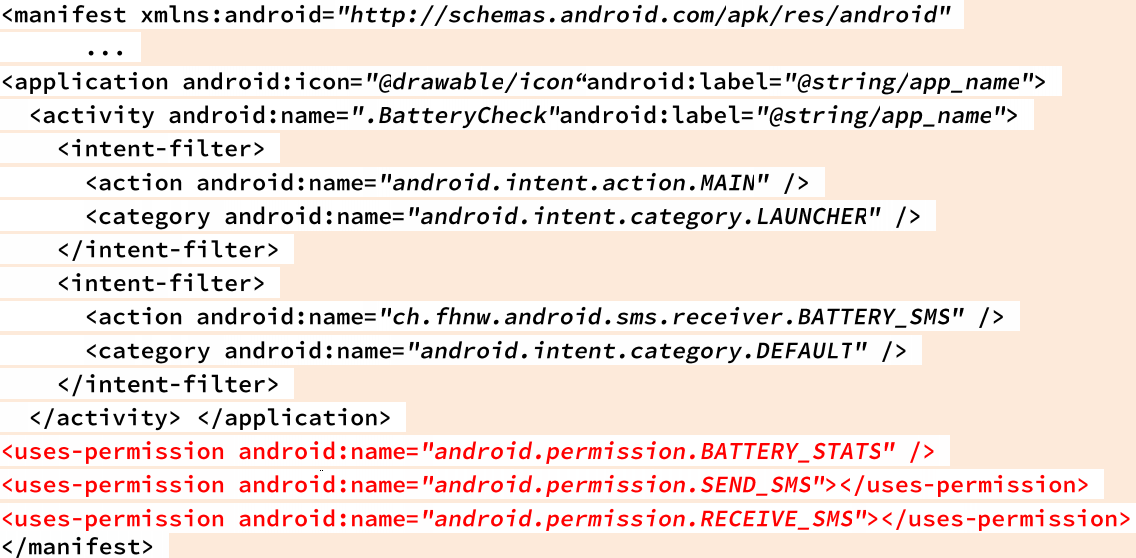
\includegraphics[scale=0.4]{AndroidManifest.png}
\end{center}
\begin{itemize}
	\item Components can be public or private (exported attribute). It specifies whether the activity can be launched by components of other applications. Default value is not reliable, set it always explicitly.
	\item If the manifest does not specify an access permission, any component in any application can access it. Components without access permissions should be exceptional cases, and possible inputs must be carefully analysed (consider splitting components). 
	\item If no permission label is set on a broadcast, any unprivileged application can read it. Always specify an access permission on Intent broadcasts (unless you specify the destination explicitly). 
\end{itemize}
\lstinputlisting[caption=Intent broadcast permissions,style=JavaStyle]{intent_broadcast_ex.java}
Android content provider permissions
\begin{itemize}
	\item seperate "read and "write"
	\item URI permissions to specify which data subsets of the parent content provider permission can be granted for
	\item Always define separate read and write permissions. Use URI permissions to delegate right to other components.
\end{itemize}
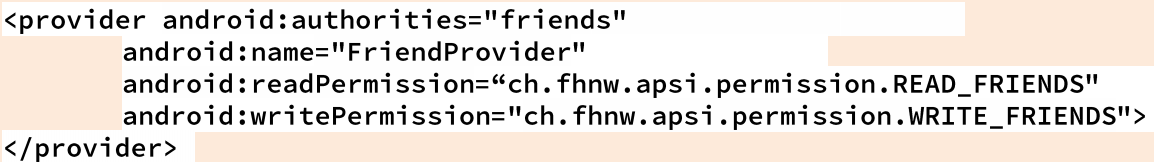
\includegraphics[scale=0.4]{content_prov_perm.png}
\begin{itemize}
	\item The application developer can add reference monitor hooks
	\item Use checkCallingPermission() to mediate "administrative" operations. Alternatively, create separate Services.
\end{itemize}
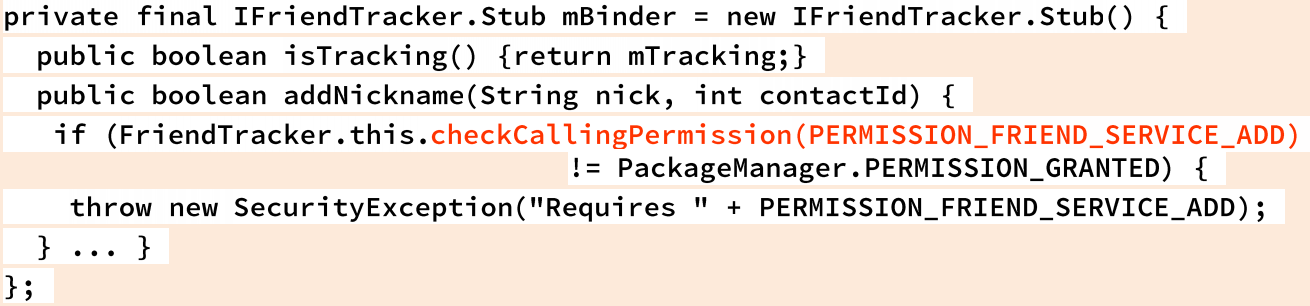
\includegraphics[scale=0.4]{service_hooks.png}
\textbf{Permission categories}: normal, dangerous, signature, signatureOrSystem
\begin{itemize}
	\item Use signature permissions for dangerous permissions. Otherwise and always include informative descriptions
\end{itemize}
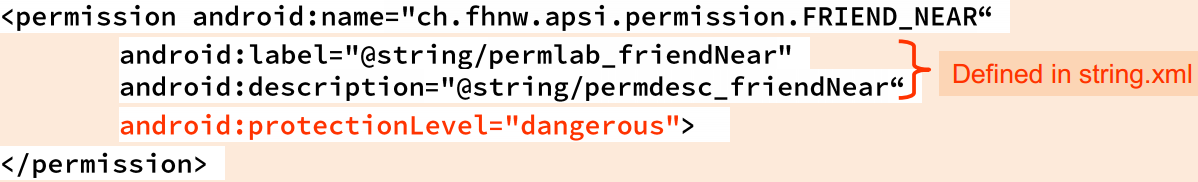
\includegraphics[scale=0.4]{perm_categ.png}
% Inhalt Ende 
\end{document} 